%!TEX root = main.tex
\section{Additional Experiments: Numerical Counterexample to Oja Convergence with Constant Step Size}
\label{sec:counter}
 \begin{figure}[!ht]
\centering
  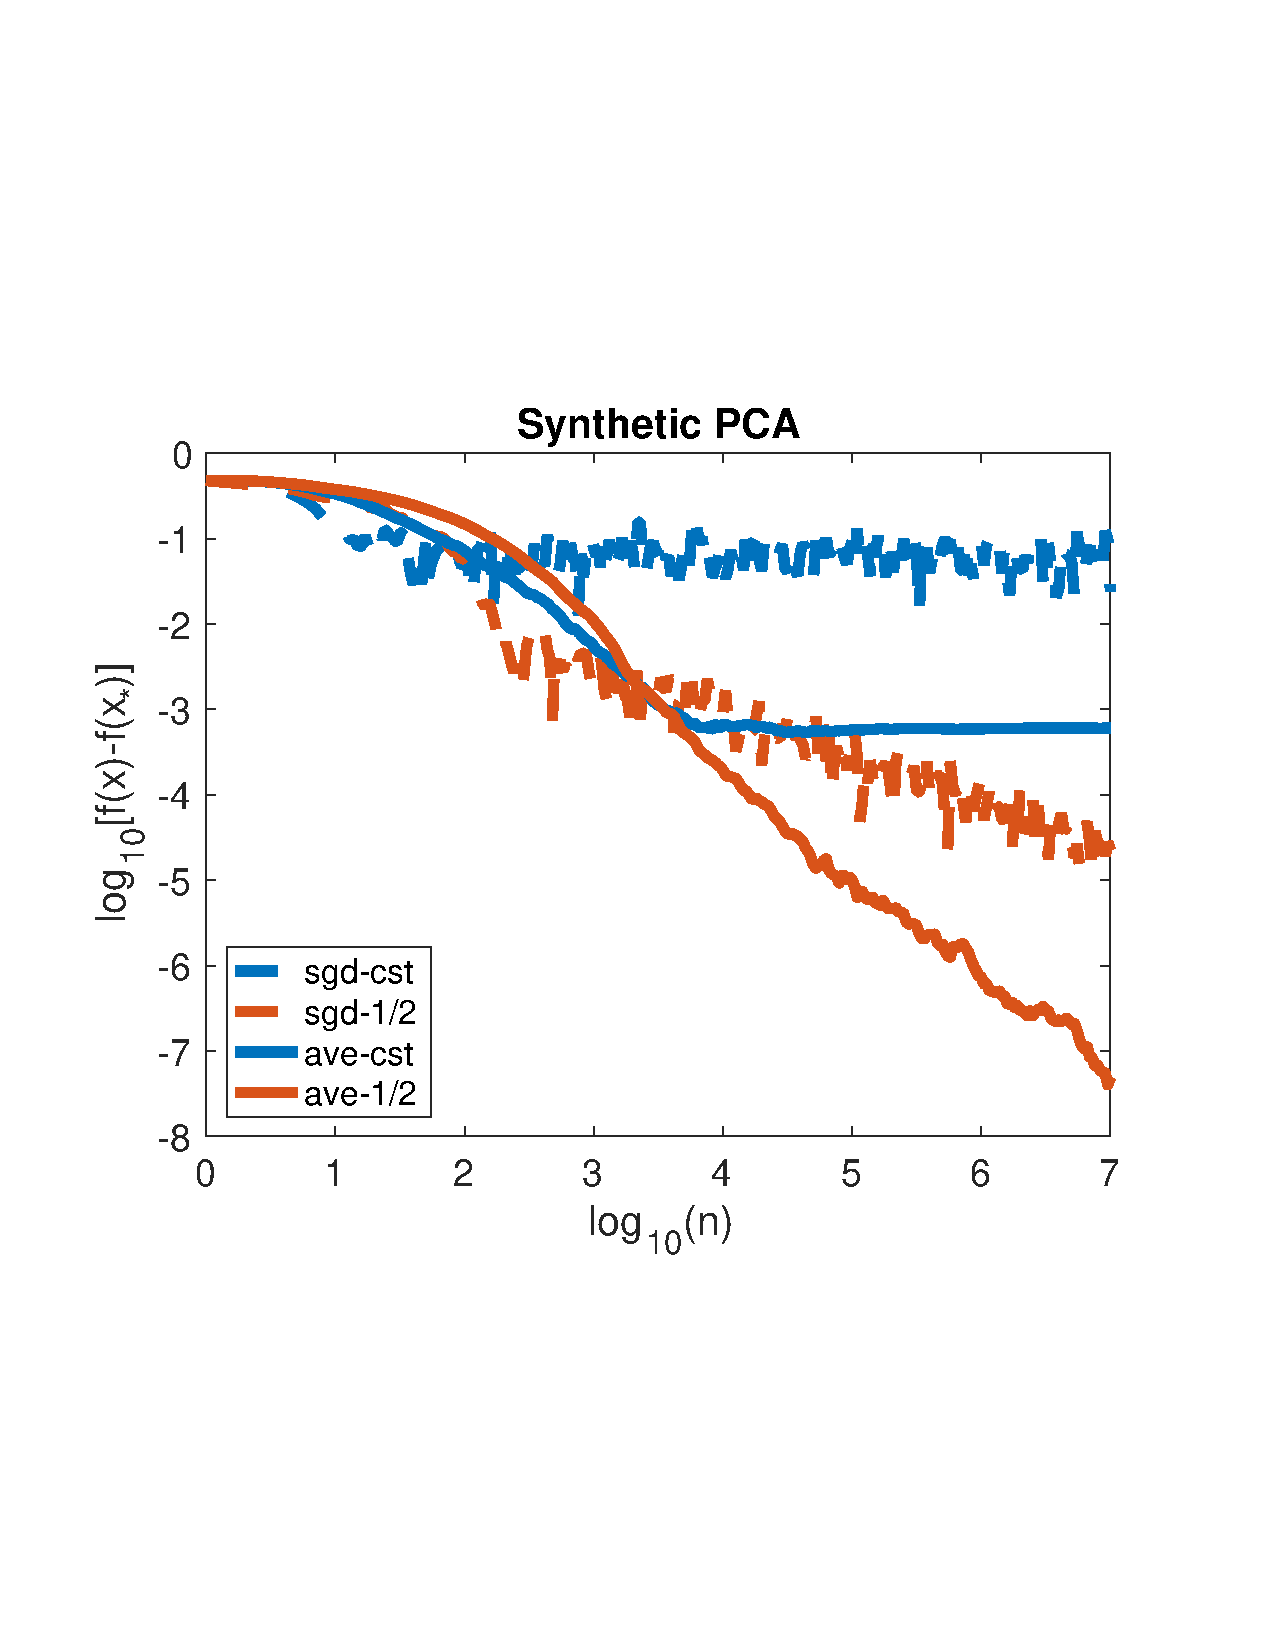
\includegraphics[width=0.8\linewidth]{Figs/counter2.pdf}
  \vspace{-3.0cm}
  \caption{Counterexample for the convergence of averaged SGD with constant step size.}
     \label{fig:counter}
\end{figure}
In this section we present an additional experiment which shows empirically that averaged SGD with constant step-size does not always converge for the streaming $k$-PCA problem. We consider $d=2$ and  a covariance matrice $H$ with random eigenvectors and two eigenvalues $\frac{1\pm1/\pi}{4}$. The noise distribution of the stream $\{h_n h_n^\top \}_{n\geq0}$ uses a more involved construction. Consider $\alpha_n\sim\mathcal N(-\pi/2,\pi^2/4)$ and $\beta_n\sim\mathcal N(\pi/4,\pi^2/16)$ and $\tau_n\sim \mathcal{B}(1/2)$. Then define $\theta_n$ as:
\[
\theta_n= \tau_n \alpha_n+(1-\tau_n)\beta_n,
\]
and the stream $h_n$ to be
\[
h_n= \Big[\frac{\cos(\theta_n)}{\sqrt{(1-1/\pi)/2}}, \frac{\sin(\theta_n)}{\sqrt{(1+1/\pi)/2}}\Big].
\]
\myfig{counter}, compares the performance of averaged SGD with constant step size $\gamma=1$ and the decreasing step size $\gamma_n=\frac{1}{\sqrt{n}}$. We see that with constant step size both SGD and averaged SGD do not converge to the true solution. SGD oscillates around the solution in ball of radius $\sim \gamma$ and averaged SGD does converge but not to the correct solution (although is still contained in a ball of radius $\sim 10^{-4}$ around the correct solution). On the other hand, SGD with decreasing step size behaves just as well as with a Gaussian data stream. SGD converges to the solution at the slow rate $O(1/\sqrt{n})$, while averaged SGD converges at the fast rate $O(1/{n})$.

This interesting example shows that constant step size averaged SGD does not converge to the correct solution in all situations. However, it remains a open problem to investigate the convergence properties of constant step size SGD in the Gaussian case.
